\documentclass[twocolumn]{d-abst}
\usepackage[dvipdfmx]{graphicx}
\graphicspath{{figs/}}
% Add period after section number
\usepackage{secdot}
\sectiondot{section}

\title{論文題目}
\author{学生氏名、指導教員名}
\keywords{キーワード 5つ}

\begin{document}

\pagestyle{empty}
\maketitle
\thispagestyle{empty}
\sloppy

\section{はじめに}

本稿は2019年度大学院入学試験(博士課程)口述試験概要のテンプレートである.
2020年度以降の書式とは乖離しているかもしれないので,注意して利用されたい.

\subsection{句読点の変換方法}

本稿における「、」や「。」は、\verb|make pub|を実行することで、「,」や「.」に変更される。

\subsection{図の貼り方}

図は\figref{nowprinting}や\tabref{sample}として参照する.

\begin{figure}[tbh]
 \begin{center}
  \begin{minipage}{0.3\columnwidth}
   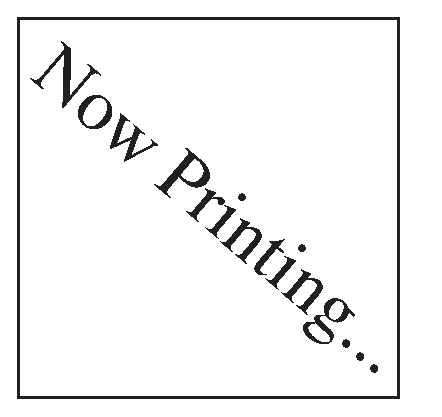
\includegraphics[width=\columnwidth]{nowprinting.eps}
   \caption{Example of eps.}
  \end{minipage}
  \hspace{0.15\columnwidth}
  \begin{minipage}{0.3\columnwidth}
   
\includegraphics[width=\columnwidth]{dj.jpg}
   \caption{Example of jpg.}
  \end{minipage}
  \label{figure:nowprinting}
 \end{center}
\end{figure}

\begin{table}[tbh]
 \begin{center}
  \begin{tabular}{|l|r|} \hline
  A1 & B1 \\
  A2 & B2 \\ \hline
  \end{tabular}
  \caption{Example of table.}
  \label{table:sample}
 \end{center}
\end{table}

\subsection{参考文献の引用方法}

\cite{launder1975progress},\cite{mitsuishi1992user},\cite{mitsuishi1995neural,timoshenko1962theory}のように引用できる.

\section{おわりに}

2019年度大学院入学試験(博士課程)口述試験概要のテンプレートを作った.

\bibliographystyle{d-abst}
\bibliography{main}

\end{document}

